\documentclass{article}

\usepackage[T2A]{fontenc}
\usepackage[utf8]{inputenc}
\usepackage[russian]{babel}
\usepackage{amsmath}
\usepackage{amssymb}
\usepackage{amsthm}
\usepackage{mathrsfs}
\usepackage{hyperref}
\usepackage{booktabs}
\usepackage{multirow}
\usepackage{makecell}
\usepackage{tabularx}
\usepackage{float}
\usepackage{amsmath,amssymb,mathtools}
\usepackage{algorithm}
\usepackage{algpseudocode}
\usepackage[normalem]{ulem}

\usepackage{dan2e}

\makeatletter
\@ifundefined{@Russian}{\newif\if@Russian \@Russiantrue}{}
\@ifundefined{@TVP}     {\newif\if@TVP    \@TVPfalse}{}
\makeatother

% ---------- Algorithmic styling ----------
\algrenewcommand\algorithmicrequire{\textbf{Require:}}
\algrenewcommand\algorithmicensure{\textbf{Ensure:}}
\algrenewcommand\algorithmicforall{\textbf{for each}}
\algrenewcommand\algorithmiccomment[1]{\hfill\(\triangleright\)~#1}

% ---------- Helpers ----------
\newcommand{\Group}{\mathrm{Group}}
\newcommand{\Concat}{\mathrm{Concat}}
\newcommand{\norm}{\mathrm{norm}}

\begin{document}
\raggedbottom
\Volume{505}
\Year{2025}
\Pages{46--49}

\udk{517.54}

\title{Реферирование художественной литературы посредством больших языковых моделей}

\author{Д.\,А.~Григорьев\Addressmark[1]\Emailmark[1], Д.\,И.~Чернышев\Addressmark[1]\Emailmark[2]}

\Addresstext[1]{Московский государственный университет им.~М.\,В.~Ломоносова, Москва, Россия}

\Emailtext[1]{dagrig14@yandex.ru}
\Emailtext[2]{chdanorbis@yandex.ru}

\markboth{Д.\,А.~Григорьев, Д.\,И.~Чернышев}{Оценка общих и специальных знаний в больших языковых моделях}

\presentedby{Представлено кем-то}

\dateA{16.08.2025}
\dateB{20.08.2025}
\dateC{31.08.2025}

\alttitle{Evaluating general and special knowledge in large language models for Russian language through replication of encyclopedia articles}

\altauthor{D.\,A.~Grigoriev\Addressmark[a]\Emailmark[1], D.\,I.~Chernyshev\Addressmark[a]\Emailmark[2]}

\altAddresstext[a]{Lomonosov Moscow State University, Moscow Center for Fundamental and Applied Mathematics, \\ Moscow, Russian Federation}

\altpresentedby{man who sold the world}


\maketitle
\doi{10.31857/S2686954322040117}

\begin{abstract}
Работа исследует методы сжатия художественных текстов с помощью языковых моделей и предлагает улучшенные подходы для точного реферирования в условиях ограниченного контекста.
\end{abstract}

\begin{keywords}
LLM, реферирование, литература, книги, краткий пересказ
\end{keywords}

\begin{altabstract}
This work explores methods for compressing literary texts using language models and proposes improved approaches for accurate summarization under limited context conditions.
\end{altabstract}

\begin{altkeywords}
LLM, summarization, literature, books, brief retelling
\end{altkeywords}


% ================= ВВЕДЕНИЕ =================
\section*{Введение}
\subsection*{Реферирование художественной литературы}
Автоматическое реферирование текста — одна из ключевых задач в области обработки естественного языка. Суть этой задачи заключается в создании информативной аннотации исходного текста с сохранением основного смысла содержания. 
В последние годы, с появлением больших языковых моделей, резко возрос интерес к автоматизации реферирования в самых разных жанрах текстов, включая художественные произведения. 
В отличие от научных, новостных или технических текстов, художественные произведения характеризуются высокой степенью стилистической и семантической сложности. 
Нелинейность повествования, образность, метафоричность и стилистические приёмы делают задачу написания краткого содержания особенно трудоёмкой. 
Ограниченное контекстное окно современных моделей дополнительно осложняет работу с длинными произведениями.

Теоретически автоматическое реферирование может выполняться двумя основными способами: экстрактивным реферированием (выбор ключевых фрагментов текста) и абстрактивным (генерация нового текста на основе содержания оригинала). 
% Поправить
Для художественной литературы более уместен второй подход, поскольку он позволяет передать смысл и стиль произведения, не нарушая его целостности.

% ================= НАБОР ДАННЫХ =================

\section*{Набор данных}
На момент начала исследования не существовало открытых и репрезентативных корпусов, предназначенных специально для задачи реферирования художественных текстов на русском языке. С целью проведения экспериментов и оценки различных подходов к генерации аннотаций был создан собственный корпус, состоящий из художественных текстов и соответствующих кратких пересказов. 
В качестве источника рефератов был выбран ресурс «Народный Брифли»~\cite{Briefly} — платформа, где пользователи публикуют краткие пересказы литературных произведений. 
Несмотря на вариативность качества и стиля пользовательских аннотаций и наличие нерелевантной информации, такой как учебные вопросы или редакторские замечания, после тщательной предварительной обработки удалось получить достаточно надёжный и чистый набор данных.
Художественные тексты были отобраны из электронной библиотеки LibRuSec — одного из крупнейших русскоязычных ресурсов художественной литературы. 
Отбор произведений осуществлялся на основании наличия аннотаций на выбранном ресурсе \cite{Briefly}. Каждый текст проходил автоматическую предварительную обработку: удалялась метаинформация (например, заголовки, описания глав и технические вставки), 
после чего текст форматировался в единый стандартизированный вид, подходящий для дальнейшего использования в моделях. 

Чтобы более точно связать книги с их аннотациями использовалось семантическое сходство: текст имени автора, записанный на Брифли и автора с LibRuSec переводился в эмбеддинги с использованием библиотеки SentenceTransformer
с помощью языковой модели\footnote{https://huggingface.co/deepvk/USER-bge-m3}
и сравнивался по косинусному сходству.
\begin{figure}[!htbp]
    \centering
    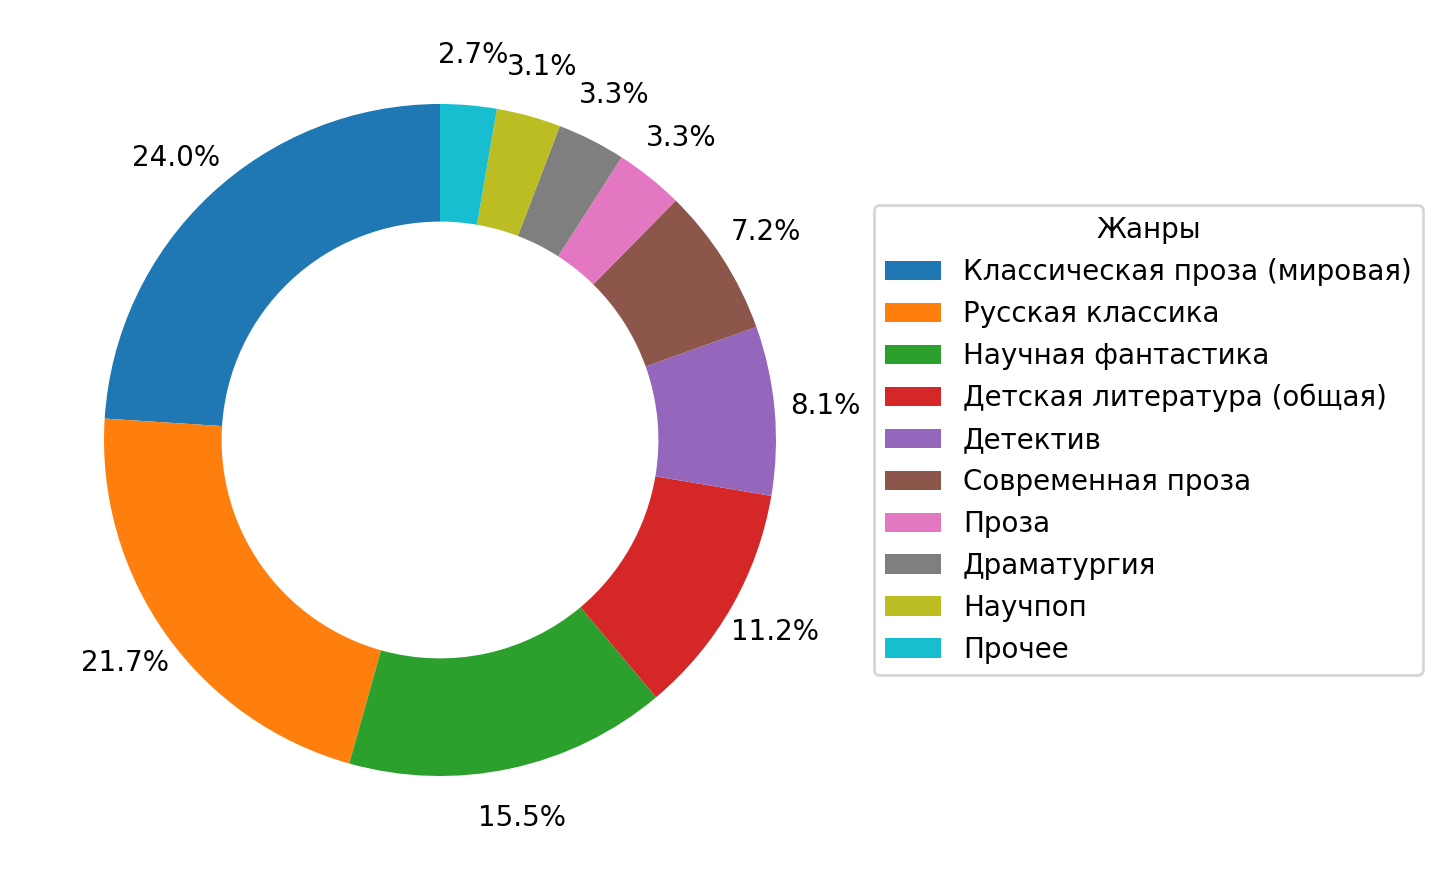
\includegraphics[width=\linewidth]{figures/genres_pie.png}
    \caption{Распределение текстов по жанрам (топ 10 жанров)}
    \label{fig:genres}
\end{figure}

\begin{table}[ht]
\centering
\caption{Обзор датасетов}
\label{tab:dataset_info}
\begin{tabular}{l|cccc}
\toprule
\textbf{Датасет} & \makecell{Число документов} & \makecell{Средняя длина \\ документа \\ (\# слов)} & \makecell{Средняя длина \\ реферата \\ (\# слов)} & \makecell{Степень сжатия \\ (длина текста \\/ длина реферата)} \\
\midrule
\textbf{RuBookSum}  & 634 & 35052.64 & 700.77 & 0.0843 \\
\hline
BookSum    & 405 & 112885.15 & 1167.20 & 0.0079 \\
Gazeta     & 60964 & 632.77 & 41.94 & 0.0699 \\
\bottomrule
\end{tabular}
\end{table}

Важно отметить, что при создании корпуса использовались только тексты, находящиеся в общественном достоянии или распространяемые свободно с разрешения правообладателей, что обеспечивает соблюдение требований авторского права.
Тексты аннотаций проходили автоматическую очистку от HTML‑тегов, комментариев и служебных пометок с помощью LLM~Meta--Llama~3--70B--Instruct. Затем производился поиск по датасету LibRuSec и собиралась коллекция, состоящая из пар "текст книги - аннотация".
\\Получившийся корпус включает в себя:
\begin{itemize}
  \item более 600 пользовательских пересказов с ресурса «Народный Брифли»;
  \item исходные произведения из электронной библиотеки LibRuSec;
\end{itemize}

На рисунке \ref{fig:genres} показано жанровое разнообразие текстов. В таблице \ref{tab:dataset_info} приведена общая информация о датасете в сравнении с аналогами.

% ================= ПРИМЕНЕНИЕ МЕТОДОВ =================
\section*{Методология}
\subsection*{Базовые и модифицированные стратегии.}

\subsubsection*{Иерархический метод. (Algorithm 1)}
Суть этого метода \cite{hierarchical} заключается в том, что текст разбивается на фрагменты (чанки), для каждого из
которых отдельно генерируется локальная аннотация. 
Эти фрагменты затем объединяются в группы, и из полученных аннотаций снова формируется краткое содержание
следующего уровня. Последний уровень представляет собой итоговый реферат всего произведения.

\subsubsection*{Иерархический метод с фильтрацией узлов. (Algorithm 2)}
Классический иерархический метод строит итоговый реферат путём многослойного объединения промежуточных рефератов, полученных из отдельных фрагментов текста. 
Однако в литературных произведениях часто встречаются фрагменты, которые не оказывают большого влияния на развитие сюжета и содержат множество избыточных
повторов и второстепенной информации. Эти фрагменты при генерации итоговой аннотации могут снижать её информативность, а в некоторых случаях даже мешать модели на этапе реферирования отдельных фрагментов.

Чтобы решить эту проблему, в метод была имплементирована фильтрация узлов по семантической близости. 
Для исключения малоинформативных или дублирующих фрагментов на каждом уровне иерархии выполняется глобальная проверка семантической близости между всеми промежуточными рефератами. 
Фрагменты, близкие по косинусной мере с предыдущими, считаются избыточными и не используются при составлении реферата на текущем уровне.
Эмбеддинги получаются с помощью SentenceTransformer (модель USER-bge-m3) и при вычислении на GPU обеспечивается высокая скорость обработки.
Эта модификация направлена на ускорение генерации за счет удаления потенциально излишних частей информации, что повышает плотность полезной информации в итоговых рефератах. 

\noindent
\begin{minipage}[t]{0.49\textwidth}
  \begin{algorithm}[H]
  \caption{Иерархический метод}
    \begin{algorithmic}
      \Require $W$ - контекстное окно модели, $D$ - входной текст, длиной $L \gg W$, $p_\theta$ - модель, $C$ - длина чанка
      \State Разбить $D$ на чанки $c_1\dots c_{\lceil \frac{L}{C} \rceil}$
      \For{$c_i=c_1\dots c_{\lceil \frac{L}{C} \rceil}$}
        \State $S_0 \gets SummarizeChunk(p_\theta, c_i)$\
      \EndFor
      \Repeat
        \State $Groups \gets GroupSummaries(S_l)$
        \State $\ell \gets \ell + 1$
        \For{$g \in Groups$}
          \State $S_l \gets \{MergeGroup(p_\theta,g)\}$
        \EndFor
      \Until{$|S_l|=1$}
      \State \Return $S_l[1]$
    \end{algorithmic}
  \end{algorithm}
\end{minipage}\hfill
\begin{minipage}[t]{0.49\textwidth}
  \begin{algorithm}[H]
    \caption{Иерархический метод с фильтрацией}
    \begin{algorithmic}
      \Require $W$ - контекстное окно модели, $D$ - входной текст, длиной $L \gg W$, $p_\theta$ - модель, $\theta$ - порог сходства, $C$ - длина чанка
      \State Разбить $D$ на чанки $c_1\dots c_{\lceil \frac{L}{C} \rceil}$
      \State $S_0 \gets \{c_1\dots c_{\lceil \frac{L}{C} \rceil}\}$
      \Repeat
        \For{$s_i \in S_l$}
          \State $e_i \gets Encoder(s_i)$
          \State $M_{ij} \gets \dfrac{\mathbf{e}_i\cdot \mathbf{e}_j}{\|\mathbf{e}_i\|\,\|\mathbf{e}_j\|}$\Comment{Матрица эмбеддингов}
          \State{Вычисляется максимальное сходство}
        \State{с предыдущими рефератами.}
          \State $m_j=\max_{i<j} M_{ji}$
          \State $S_l \gets \{s_i \mid m_i < \theta$ \textbf{ or } $i = 0 \}$ \Comment{Фильтрация}
        \EndFor
        \State $Groups \gets GroupSummaries(S_l)$
        \State $\ell \gets \ell + 1$
        \For{$g \in Groups$}
          \State $S_l \gets \{MergeGroup(p_\theta,g)\}$
        \EndFor
      \Until{$|S_l|=1$}
      \State \Return $S_l[1]$
    \end{algorithmic}
  \end{algorithm}
\end{minipage}

\vspace{0.4em}
\subsubsection*{«Чертёжный» метод (Text‑Blueprint). (Algorithm 3)}
Данный метод \cite{blueprint} по сути является модификацией иерархического и ориентирован на построение промежуточного
плана аннотации перед генерацией текста. План формируется в виде набора вопросноответных пар, что повышает управляемость генерации и обеспечивает структурированность результата.
Сначала модель формирует список вопросов, отражающих ключевые события, темы
и персонажей текста. Далее к каждому вопросу автоматически подбирается краткий
ответ. Эта структура служит планом, по которому генерируется итоговая аннотация.


\subsubsection*{«Чертёжный» метод с кластеризацией вопросов. (Algorithm 4)}
Базовая реализация «чертёжного» метода предполагает генерацию вопросно-ответного
плана для каждого фрагмента текста и каждого уровня объединения аннотаций. Однако при работе с художественными текстами вопросы, генерируемые для каждого чанка,
могут сбивать агрегацию текста моделью, делая аннотацию менее структурированной
и содержательно полной. К тому же, генерация плана на каждом шаге алгоритма существенно замедляет его работу и использует дополнительные мощности языковых моделей.
Для снижения числа запросов к модели и повышения структурности, была добавлена кластеризация вопросов с использованием SentenceTransformers и алгоритма K-means.

\noindent
\begin{minipage}[t]{0.49\textwidth}
  \begin{algorithm}[H]
    \caption{<<Чертежный>> метод}
    \begin{algorithmic}
      \Require $W$ - контекстное окно модели, $D$ - входной текст, длиной $L \gg W$, $p_\theta$ - модель, $C$ - длина чанка, $R$ - ограничение по длине
      \State Разбить $D$ на чанки $c_1\dots c_{\lceil \frac{L}{C} \rceil}$
      \For{$c_i=c_1\dots c_{\lceil \frac{L}{C} \rceil}$}
        \State $b_i \gets GenerateBlueprint(p_\theta, c_i)$\
        \State $S_0 \gets \{SummarizeWithBp(p_\theta, b_i, c_i)\}$\
      \EndFor
      \Repeat \Comment{Объединение рефератов}
        \State $Groups \gets GroupSummaries(S_l)$
        \State $\ell \gets \ell + 1$
        \For{$g \in Groups$}
          \If{$Length(g) > R$}
            \State $b_i \gets GenerateBlueprint(p_\theta, g)$\
            \State $S_l \gets \{SummarizeWithBp(p_\theta, b_i, g)\}$\
          \Else
            \State $S_l \gets \{g\}$\
          \EndIf
        \EndFor
      \Until{$|S_l|=1$}
      \State \Return $S_l[1]$
    \end{algorithmic}
  \end{algorithm}
\end{minipage}\hfill
\begin{minipage}[t]{0.49\textwidth}
  \begin{algorithm}[H]
  \caption{<<Чертежный>> метод с кластеризацией}
      \begin{algorithmic}
        \Require $W$ - контекстное окно модели, $D$ - входной текст, длиной $L \gg W$, $p_\theta$ - модель, $C$ - длина чанка, $R$ - ограничение по длине
        \State Разбить $D$ на чанки $c_1\dots c_{\lceil \frac{L}{C} \rceil}$
        \For{$c_i=c_1\dots c_{\lceil \frac{L}{C} \rceil}$}
          \State $b_i \gets GenerateBlueprint(p_\theta, c_i)$
          \State $Q \gets \{ExtractQuestions(p_\theta, b_i)\}$
        \EndFor
        \For{$q_i \in Q$}
          \State $E \gets \{Encoder(q_i)\}$
          \State $K \gets KMeans(E)$
          \For{$k_i \in K$}
            \State $q_i \gets Generalize(p_\theta, k_i)$
            \State $Q \gets \{q_i\}$ \Comment{Собирается общий план}
          \EndFor
          \For{$c_i=c_1\dots c_{\lceil \frac{L}{C} \rceil}$}
            \State $S_0 \gets \{SummarizeWithBp(p_\theta, b_i, c_i)\}$\
          \EndFor
        \EndFor
        \State \textbf{Объединение рефератов} аналогично <<Чертежному методу>> с тем отличием что здесь в качестве чертежа используется один глобальный план Q
      \end{algorithmic}
  \end{algorithm}
\end{minipage}

Такой подход позволяет уменьшить число обращений к LLM, что позволяет ускорить скорость генераций, как будет показано в таблице \ref{tab:results_models}.

% ====================== ROW 2: Blueprint ======================


\section*{Метрики}

Для объективного сравнения описанных подходов и моделей в задаче реферирования художественных текстов использовались четыре группы метрик.

\textbf{ROUGE-L} — основана на длине наибольшей общей подпоследовательности (LCS) между сгенерированной аннотацией $S$ и эталонной $R$:
    \[
      \text{Precision} = \frac{\mathrm{LCS}(S,R)}{|S|},\quad
      \text{Recall} = \frac{\mathrm{LCS}(S,R)}{|R|},
    \]
    \[
      \text{ROUGE‑L} = \frac{2\;\text{Precision}\;\cdot\;\text{Recall}}{\text{Precision} + \text{Recall}}.
    \]
\\ \textbf{BERTScore} — семантическое качество на уровне токенов. Для каждой пары токенов предсказания и эталона вычисляется косинусное сходство их эмбеддингов в модели USER‑bge‑m3. Затем:
    \[
      P = \frac{1}{|S|}\sum_{t\in S}\max_{u\in R}\!\mathrm{sim}(e_t, e_u),\quad
      R = \frac{1}{|R|}\sum_{u\in R}\max_{t\in S}\!\mathrm{sim}(e_u, e_t),
    \]
    \[
      \text{BERTScore} = \frac{2\,P\,R}{P+R}.
    \]
\\ \textbf{Полнота покрытия ключевых вопросов (Coverage)} — доля заранее сгенерированных по эталонному тексту вопросов, на которые модель «отвечает» в аннотации:
    \[
      \text{Coverage} = \frac{\#\{q_i\colon P(\text{“да”}\mid q_i,S)\!>\!0.75\}}{N},
    \]
    где $N$ — общее число вопросов, а $P(\text{“да”}\mid q_i,S)$ — вероятность наличия ответа на вопрос $q_i$ в тексте $S$, оцененная LLM.
\\ \textbf{Совпадение ответов (AnswerSimilarity)} — среднее семантическое сходство между сгенерированными ответами $a_i^{\text{pred}}$ и эталонными $a_i^{\text{ref}}$ на те же ключевые вопросы:
    \[
      \text{AnswerSimilarity}
      = \frac{1}{N}\sum_{i=1}^N \mathrm{sim}\bigl(a_i^{\text{pred}},\,a_i^{\text{ref}}\bigr),
    \]
    где $\mathrm{sim}$ — косинусное сходство эмбеддингов, полученных через USER‑bge‑m3.


Использование нескольких метрик, учитывающих как поверхностное совпадение текста, так и глубокое семантическое сходство (BERTScore, AnswerSimilarity), а также степень охвата заранее заданных вопросов (Coverage), обеспечивает всестороннюю и устойчивую оценку качества аннотаций.

\section*{Параметры экспериментов}

Все представленные в работе измерения выполнены на тестовой части датасета, 
отобранных так, чтобы исходные тексты не превышали по длине 800\,000 символов. 
Для всех методов генерируемые аннотации ограничивались максимумом в 500 слов.

Текст на вход разбивался на чанки фиксированного размера в 2000 токенов. 
Токенизация выполнялась с помощью \texttt{AutoTokenizer} модели \texttt{DeepPavlov/rubert-base-cased} в стандартном режиме.
Для воспроизводимости всех случайных процедур использовался фиксированный seed ($random\_seed = 42$).

В \textbf{иерархическом методе с фильтрацией узлов} для оценки избыточности промежуточных рефератов на каждом уровне вычислялась матрица косинусных сходств между их эмбеддингами.
Порог схожести был установлен равным $\theta=0.85$: если для аннотации $S_j$ существует предыдущая $S_i$ с косинусным сходством выше этого порога, 
то $S_j$ отбрасывается как избыточная. Такой выбор порога обеспечивает компромисс между сохранением значимой информации и устранением дублирования, 
что эмпирически привело к заметному уменьшению объёма промежуточных представлений без существенной деградации качества.

В \textbf{чертёжном методе с кластеризацией вопросов} количество кластеров для K-means выбирается по эвристике, подобранной эмпирически:
\[
n_{\text{clusters}} = \max\!\left(2,\; \left\lceil \sqrt{N_{\text{questions}}} \right\rceil\right),
\]
где $N_{\text{questions}}$ — общее число сгенерированных вопросов по всем чанкам до кластеризации. 
Гарантируется минимум в два кластера, что позволяет даже при небольших наборах вопросов получать структурированное чертёжное представление.

Временные показатели измерялись как среднее значение (в секундах) времени генерации одной книги по каждому методу для 100 книг. 
В случае всех четырех методов учитывалось суммарное время всех этапов (включая генерацию промежуточных аннотаций / планов, фильтрацию и финальную агрегацию).

\section*{Результаты}
\subsection*{Замеры времени.}
Проводились первоначальные замеры скорости работы методов на небольших текстах, полученные результаты в секундах (среднее по трем запускам) представлены в таблице \ref{tab:timing}. 
Результаты подтверждают, что модификации позволяют повысить скорость генерации.
\begin{table}[ht]
\centering
\caption{Время генерации аннотации (в секундах) для текста размером 81{,}049 символов (11 чанков). Усреднено по трём запускам.}
\label{tab:timing}
\begin{tabular}{lcccc}
\toprule
\textbf{Модель} & \makecell{Иерархический} & \makecell{Иерархический\\с фильтрацией} & \makecell{Чертежный} & \makecell{Чертежный\\с кластеризацией} \\
\midrule
RuadaptQwen2.5-7B-Lite-Beta  & 84.64 & 25.70 & 103.66 & 78.99 \\
RuadaptQwen3-32BInstruct-v2 & 218.23 & 72.54 & 420.95 & 470.4 \\
DeepSeek V3                  & 237.83 & 72.42 & 292.80 & 268.75 \\
Qwen3-235B-A22B              & 113.24 & 39.45 & 215.63 & 145.20 \\
tpro                         & 472.23 & 127.38 & 421.65 & 185.94 \\
yagpt5lite                   & 34.17 & 14.08 & 99.70 & 27.26 \\
\bottomrule
\end{tabular}
\end{table}

\subsection*{Полученные результаты.}
В таблице \ref{tab:results_models} представлены сравнительные метрики качества автоматического пересказа книг разными моделями и методами обработки. Для каждой комбинации модели и метода измерялись BERTScore, ROUGEL, Answer Coverage и 
Similarity, а также время генерации (среднее) на 100 примерах, одинаковых для всех замеров. Лучше всего себя показала модель Qwen3-\allowbreak 235B-\allowbreak A22B: она продемонстировала самые высокие показатели в покрытие вопросов и сходстве ответов.
В то же время важно отметить, что среди всех методов лучшим образом в соотношение качество и время обработки себя показывает иерархический метод с фильтрацией узлов. Он позволяет существенно ускорить время обработки (например, почти в два раза для модели DeepSeek V3), и по сравнению с 
чертежным методом, который в среднем показывал лучшие результаты, не сильно отстает по показателям. Исключением стала лишь модель Qwen3-\allowbreak 235B-\allowbreak A22B, так как она показала лучший результат среди всех моделей на базовом чертежном методе.
Эксперименты показали, что иерархический метод с фильтрацией узлов обеспечивает наилучший компромисс между скоростью и качеством генерации.

\begin{table}[ht!]
\centering
\small
\setlength{\tabcolsep}{4pt}
\caption{Результаты по методам и моделям}
\label{tab:results_models}

\begin{tabular}{ll|c|c|c|c}
\toprule
Модель & Метрики &
\makecell{Иерархический} &
\makecell{Чертежный} &
\makecell{Иерархический \\ с фильтрацией} &
\makecell{Чертежный \\ с кластеризацией} \\
\midrule
\multirow{5}{*}{\makecell{RuadaptQwen2.5-7B\\Lite-Beta}}
 & bertscore & 55.4 ± 2.9 & 56.1 ± 4.9 & 55.8 ± 2.9 & 54.0 ± 4.0 \\
 & rouge-l   & 8.6 ± 2.5 & 10.1 ± 3.9 & 8.7 ± 2.5 & 7.7 ± 2.8 \\
 & coverage  & 19.66 ± 17.77 & 24.94 ± 21.08 & 20.31 ± 17.95 & 15.51 ± 14.83 \\
 & similarity& 15.16 ± 14.11 & 20.03 ± 17.50 & 15.94 ± 14.39 & 12.23 ± 12.30 \\
 & time      & 68.86 ± 64.85 & 126.84 ± 145.74 & 53.59 ± 47.28 & 76.66 ± 91.78 \\
\midrule
\multirow{5}{*}{yagpt5lite}
 & bertscore & 62.5 ± 3.5 & 61.1 ± 3.8 & 62.1 ± 3.2 & 61.5 ± 3.3 \\
 & rouge-l   & 16.9 ± 5.1 & 15.8 ± 5.1 & 16.4 ± 4.7 & 14.3 ± 4.4 \\
 & coverage  & 36.85 ± 19.40 & 33.17 ± 21.58 & 31.75 ± 20.06 & 24.28 ± 16.95 \\
 & similarity& 29.69 ± 16.43 & 26.58 ± 18.13 & 25.60 ± 16.85 & 19.70 ± 14.29 \\
 & time      & 31.02 ± 28.51 & 113.34 ± 123.78 & 27.39 ± 28.05 & 42.15 ± 56.50 \\
\midrule
\multirow{5}{*}{\makecell{RuadaptQwen3-32B\\Instruct-v2}}
 & bertscore & 57.3 ± 2.9 & 58.9 ± 3.6 & 57.7 ± 3.3 & 55.3 ± 3.3 \\
 & rouge-l   & 11.0 ± 2.4 & 10.6 ± 3.2 & 10.7 ± 2.4 & 7.8 ± 2.1 \\
 & coverage  & 33.12 ± 21.50 & 33.18 ± 22.83 & 32.19 ± 22.52 & 17.72 ± 15.23 \\
 & similarity& 25.25 ± 16.94 & 26.21 ± 18.22 & 24.82 ± 17.74 & 13.97 ± 12.39 \\
 & time      & 218.30 ± 195.16 & 379.24 ± 500.40 & 166.79 ± 164.61 & 286.35 ± 395.97 \\
\midrule
\multirow{5}{*}{tpro}
 & bertscore & 59.4 ± 3.0 & 59.0 ± 4.9 & 59.5 ± 3.3 & 58.2 ± 3.7 \\
 & rouge-l   & 13.8 ± 3.1 & 14.7 ± 4.9 & 13.5 ± 3.0 & 11.8 ± 3.9 \\
 & coverage  & 40.27 ± 20.23 & 40.83 ± 22.42 & 37.13 ± 20.72 & 26.03 ± 18.44 \\
 & similarity& 31.77 ± 16.63 & 32.60 ± 18.57 & 29.44 ± 16.83 & 20.83 ± 15.26 \\
 & time      & 367.32 ± 324.49 & 592.39 ± 772.19 & 267.73 ± 253.34 & 247.59 ± 361.20 \\
 \midrule
\multirow{5}{*}{Qwen3-235B-A22B}
 & bertscore & 61.2 ± 3.0 & 61.6 ± 3.3 & 60.9 ± 2.7 & 59.3 ± 3.4 \\
 & rouge-l   & 14.9 ± 4.0 & 15.8 ± 4.5 & 14.8 ± 3.7 & 12.2 ± 3.6 \\
 & coverage  & 52.48 ± 20.79 & \textbf{54.78 ± 21.16} & 44.54 ± 23.03 & 30.19 ± 21.96 \\
 & similarity& 41.68 ± 17.18 & 43.99 ± 17.54 & 35.67 ± 18.87 & 24.10 ± 17.62 \\
 & time      & 103.49 ± 97.30 & 230.35 ± 271.03 & 83.06 ± 102.05 & 158.30 ± 196.35 \\
\midrule
\multirow{5}{*}{DeepSeek V3}
 & bertscore & 60.0 ± 3.1 & 58.0 ± 4.0 & 60.0 ± 2.9 & 58.4 ± 3.6 \\
 & rouge-l   & 13.7 ± 3.9 & 12.6 ± 4.6 & 13.5 ± 3.7 & 11.2 ± 3.9 \\
 & coverage  & \textbf{53.57 ± 21.66} & 40.19 ± 23.68 & \textbf{45.00 ± 23.03} & \textbf{34.68 ± 23.77} \\
 & similarity& 42.38 ± 17.73 & 32.31 ± 19.33 & 35.64 ± 18.88 & 27.76 ± 19.75 \\
 & time      & 196.77 ± 187.85 & 315.67 ± 321.89 & 147.21 ± 146.4 & 132.60 ± 197.25 \\
\bottomrule
\end{tabular}
\end{table}


\subsection*{Анализ и сравнение результатов.}
Разброс значений метрики QA можно проиллюстрировать на примере работы одной и той же модели (DeepSeek V3) в рамках иерархического метода.
В качестве иллюстрации взяты две аннотации к произведениям <<И грянул гром>> и <<Кастрюк>>. 
В первом случае модель получила высокий результат, ответив на все, кроме одного вопроса; во второй 
аннотации содержались ответы только на два вопроса из одиннадцати, что привело к низкому показателю. В таблице \ref{tab:annotations} показаны две аннотации. 
Для краткости в них выделены только основные моменты, которые
повлияли на итоговую метрику. 
Сравнение показывает возможную причину столь значительного расхождения: аннотация к рассказу <<Кастрюк>> содержит большое количество лирических отступлений и художественных деталей,
из-за чего суть произведения сложно уловить и модель отвлекается от фиксации главных фактов,
тогда как в "И грянул гром" события изложены последовательно и структурировано, 
а основные элементы сюжета чётко перечислены, что существенно упрощает задачу поиска важной информации.
В текстах выделены жирным шрифтом фрагменты, которые несут в себе важную сюжетную информацию, а подчеркнутый текст - то, что можно было бы опустить.
\begin{table}[ht!]
\centering
\begin{tabular}{|p{0.15\linewidth}|p{0.75\linewidth}|}
\hline
\makecell{\textbf{Название}} & \makecell{\textbf{Текст}} \\ \hline

\makecell{\textbf{И грянул} \\ \textbf{гром}} & \dots
\textbf{Главный герой, Экельс}, азартный и самоуверенный охотник, \textbf{платит} огромную сумму \textbf{за возможность отправиться на 60 миллионов лет назад, чтобы убить тираннозавра}. 
Перед путешествием гид Тревис строго предупреждает его о правилах: \textbf{ни в коем случае нельзя сходить с антигравитационной Тропы} или вмешиваться в естественный ход событий, 
так как малейшее нарушение может катастрофически изменить будущее.\dots Тревис объясняет \textbf{хрупкость временного баланса: 
даже гибель одной мыши способна уничтожить целые виды}, а значит, и изменить историю человечества. \textbf{Группа выслеживает тираннозавра}, помеченного красной краской — это знак, 
что \textbf{его убийство не повлияет на будущее}. Однако при виде гигантского хищника \textbf{Экельс впадает в панику, сходит с Тропы и случайно раздавливает бабочку}\dots 
По возвращении в 2055 \dots \textbf{мир изменился до неузнаваемости: язык стал грубым, атмосфера — тяжёлой, а вместо умеренного президента Кейта у власти стоит жестокий диктатор Дойчер.} 
Экельс осознаёт, что \textbf{его неосторожность спровоцировала «эффект бабочки»} — раздавленное насекомое вызвало цепь событий, исказивших историю. 
В отчаянии он умоляет исправить ошибку, но \textbf{Тревис, понимая необратимость последствий, поднимает ружьё.} \dots
 \\ \hline

\textbf{Кастрюк} & \dots \uline{Действие рассказа разворачивается в русской деревне ранней весной, 
где природа пробуждается, но жизнь людей остаётся тяжёлой и однообразной.} \textbf{Главный герой — старик Семён, прозванный Кастрюком}, — 
доживает свои дни в одиночестве, \textbf{терзаемый воспоминаниями о былой силе} и сожалениями о нынешней немощности. \textbf{Когда-то он славился как лучший работник в округе}, 
\uline{но теперь, дряхлый и забытый, вынужден оставаться в стороне, пока односельчане трудятся в поле}. Его единственная отрада — внучка Дашка, добрая и впечатлительная девочка, 
\uline{которая прибегает к нему, испугавшись барчуков из соседнего имения Залесное. Кастрюк успокаивает её, и они вместе отправляются за деревню, где старик, любуясь весенней природой, 
пытается отвлечься от гнетущих мыслей}. \dots
\textbf{Лишь к вечеру, уговорив сына отпустить его в ночное (пасти лошадей), Кастрюк обретает краткую радость}. \uline{На свободе, среди ребятишек и под звёздным небом, он чувствует себя почти молодым. 
У пруда кобыла пьёт воду, отражая закат,} а сам \textbf{старик, глядя на Млечный Путь, шепчет молитву — будто вновь обретает связь с миром и утраченную гармонию}. 
\uline{Но это лишь мимолётное утешение: завтра его снова ждёт беспросветное одиночество и осознание собственной ненужности.} \dots
  \\ \hline

\end{tabular}
\caption{Сравнение лучшего и худшего сгенерированного реферата}
\label{tab:annotations}
\end{table}


Переходя к сравнению между моделями, можно отметить, что в целом DeepSeek V3 показывает лучшие показатели, чем модели меньшей категории, однако, если сравнивать чертежный метод, то в 30\% случаев модель 
RuadaptQwen3-\allowbreak 32B-\allowbreak Instruct-\allowbreak v2 показывает лучшие результаты, а tpro в 43\%. Для сравнения можно взять аннотацию по произведению <<И грянул гром>>, созданную с использованием чертежного метода, 
небольшие вырезки которой приведены в таблице \ref{tab:annotations_deepseek_vs_others}.
В то время как аннотация, созданная моделью DeepSeek V3 больше похожа на перечесление основных событий через нумерованный список,
текст у моделей RuadaptQwen3-\allowbreak 32B-\allowbreak Instruct-\allowbreak v2 и tpro является связным пересказом текста, раскрывающим все основные события сюжета.

\begin{table}[htbp!]
\centering
\begin{tabular}{|p{0.15\linewidth}|p{0.75\linewidth}|}
\hline
\makecell{\textbf{Модель}} & \makecell{\textbf{Текст}} \\ \hline

\makecell{RuadaptQwen3} & "Компания «Сафари во Времени» организует платные экскурсии в прошлое для охоты на динозавров, 
используя машины времени, способные перемещаться между эпохами.  
Клиенты обязаны соблюдать строгие правила: следовать по металлической тропе\dots
 \\ \hline

\makecell{tpro} & "В тексте главный герой, Экельс, отправляется на сафари во времени с целью убить динозавра Tyrannosaurus rex. 
Компания, организующая сафари, гарантирует только динозавров и строго запрещает охотникам сходить 
с Тропы \dots
Мистер Тревис, проводник сафари, объясняет, что даже уничтожение одной мыши может привести к исчезновению всех её потомков \dots
 \\ \hline

\makecell{DeepSeek V3} & "**Краткое содержание по плану:** 1. **Экельс** — охотник \dots
 2. **Компания «Сафари во времени»** организует охоту в прошлом \dots
 3. **Тревис** — проводник, контролирующий экспедицию. \dots
  \\ \hline

\end{tabular}
\caption{Сравнение моделей при генерации рефератов по чертежному методу}
\label{tab:annotations_deepseek_vs_others}
\end{table}

Следует отметить, что лучшего результата удалось добиться именно чертежным методом с помощью большой модели Qwen3-\allowbreak 235B-\allowbreak A22B, 
как было показано в таблице \ref{tab:results_models}. Для сравнения качества аннотаций можно взять рассказ <<Барбос и Жулька>> - в иерархическом методе
модель Qwen3-\allowbreak 235B-\allowbreak A22B посчитала, что <<Жулька>> - не собака, а лошадь. Также, например, DeepSeek V3 более строго следует шаблону чертежного метода и вместо связного текста пересказа получается нумерованный список
пунктов с ключевыми событиями и главными героями. Однако Qwen3-\allowbreak 235B-\allowbreak A22B пишет обычный текст, без списков. Таким образом, чертежный метод без модификаций позволил достичь наилучшего результата с использованием лучшей доступной моделью - 
Qwen3-\allowbreak 235B-\allowbreak A22B.

% -------------------------------------------------------

\section*{Заключение}
В заключение, был создан первый открытый датасет, объединяющий тексты книг и аннотации к ним с открытого ресурса <<Народный Брифли>>. 
В работе предложены два улучшенных подхода к реферированию художественных текстов с использованием LLM: иерархический с фильтрацией и чертёжный с кластеризацией. 
Иерархический метод с фильтрацией позволяет ускорить генерацию при минимальной потере качества, 
что делает этот метод пригодным для обработки длинных произведений в условиях ограниченного контекста моделей.  

Сравнительный анализ показал, что крупные модели, такие как DeepSeek~V3 и Qwen3-\allowbreak 235B-\allowbreak A22B, в большинстве случаев обеспечивают более высокое покрытие QA и 
большую полноту аннотаций по сравнению с компактными моделями, особенно в иерархическом и чертёжном методах. 
Однако для некоторых типов текстов и методов (например, базовый чертёжный) более компактные модели, такие как RuadaptQwen3-\allowbreak 32B-\allowbreak Instruct-\allowbreak v2, 
могут демонстрировать конкурентоспособное качество при меньших вычислительных затратах. 
Таким образом, выбор модели следует определять исходя из баланса между доступными ресурсами, требованиями к качеству и характером обрабатываемых текстов.



%-------РЕФЕРЕНСЫ---------
\begin{thebibliography}{99}
\bibitem{Briefly}
\textit{Народный Брифли.}  
Электронная библиотека кратких пересказов литературных произведений.  
\url{https://wiki.briefly.ru/} (дата обращения: 16.07.2025).

\bibitem{hierarchical}
\textit{Иерархический метод.}  
Wu J. et al. Recursively Summarizing Books with Human Feedback //arXiv e-prints. – 2021. – С. arXiv: 2109.10862.

\bibitem{blueprint}
\textit{Чертежный метод.}  
Text-Blueprint: An Interactive Platform for Plan-based Conditional Generation / Fantine Huot, Joshua Maynez, Shashi Narayan et al. // Proceedings of the 17th Conference of the European Chapter of the Association for Computational Linguistics:
System Demonstrations / Ed. by Danilo Croce, Luca Soldaini. — Dubrovnik, Croatia: Association for Computational Linguistics, 2023. — . — Pp. 105–116. https:
//aclanthology.org/2023.eacl-demo.13/.



\end{thebibliography}

\renewcommand\refname{References}


\begin{thebibliography}{99}
\bibitem{Briefly_e}
\textit{Народный Брифли.}  
Электронная библиотека кратких пересказов литературных произведений.  
\url{https://wiki.briefly.ru/} (дата обращения: 16.07.2025).

\bibitem{hierarchical_e}
\textit{Иерархический метод.}  
Wu J. et al. Recursively Summarizing Books with Human Feedback //arXiv e-prints. – 2021. – С. arXiv: 2109.10862.

\bibitem{blueprint_e}
\textit{Чертежный метод.}  
Text-Blueprint: An Interactive Platform for Plan-based Conditional Generation / Fantine Huot, Joshua Maynez, Shashi Narayan et al. // Proceedings of the 17th Conference of the European Chapter of the Association for Computational Linguistics:
System Demonstrations / Ed. by Danilo Croce, Luca Soldaini. — Dubrovnik, Croatia: Association for Computational Linguistics, 2023. — . — Pp. 105–116. https:
//aclanthology.org/2023.eacl-demo.13/.

\end{thebibliography}

\end{document}